\documentclass[Thesis.tex]{subfiles}
\begin{document}
\chapter{Verification and Benchmarking}
\label{chp:verfication}

This chapter is dedicated to presenting some of the tests that we have done to
verify that the software we have developed is indeed functioning as advertised.
These types of tests are more large scale (integration tests) compared to low
level unit tests which is a part of the source code for QFLOW. By checking that
we can reproduce known benchmarks and observe behavior that is consistent with
our expectations we can increase the amount of trust assigned to the implementation.

\section{Setup}

We focus our tests on the idealized harmonic oscillator system in $D = 3$ dimensions
with $N$ non-interacting particles, i.e.\ the Hamiltonian given by
\cref{eq:ho-no-interaction-hamiltonian}:

\begin{align}
    \hat H_0 &= \sum_{i=1}^N\qty(-\frac{1}{2}\laplacian_i +
    \frac{1}{2}r_i^2),
\end{align}
where we have $\hbar = m = \omega = 1$, and
$r_i^2 = x_i^2 + y_i^2+z_i^2$. This has the ground state given by
\cref{eq:Phi-non-inter}, generalized to $N$ particles in three dimension and
omitting normalization constants:

\begin{align}
        \Phi(\mat X) &= \exp[-\frac{1}{2}\sum_{i=1}^N r_i^2],
\end{align}
where as before we have defined $\mat X$ as

\begin{align}
  \mat X &\defeq \mqty(\vx_1\\\vx_2\\\vdots\\\vx_N) \defeq \mqty(x_1&y_1&z_1\\x_2&y_2&z_2\\\vdots&\vdots&\vdots\\x_N&y_N&z_N)
\end{align}

For the trail wave function we shall use two different ones. First, the simple
Gaussian form of the ground state it self:

\begin{align}
  \psi_G(\mat X) = \exp(-\alpha\sum_{i = 1}^N r_i^2),
\end{align}
with $\alpha$ the only variational parameter. Learning the ideal parameters
should be trivial in this case, and we should expect perfect results.

Second, we use an ansatz resulting from a Gaussian-Binary Restricted Boltzmann
Machine (RBM), given in \cref{eq:rbm-def}:


\begin{align}
  \psi_{RBM}(\vX) &=
        \exp[-\sum_i^{M} \frac{\qty(X_i-a_i)^2}{2\sigma^2}]
        \prod_j^H \qty(1 + \exp[b_j+\sum_i^M \frac{X_iW_{ij}}{\sigma^2}]),
\end{align}
where $M = P\cdot D$ is the number of degrees of freedom and $H$ is
the number of hidden nodes (set to 4 through this section). Note also that $X_i$
in the above refers to the $i$'th degree of freedom, counting through $\mat X$
in row major order. The variational parameters are $\vb a, \vb b$ and $\mat W$,
and we hold $\sigma^2=1$ constant in this case.

We use this wave function simply to make learning the true ground state slightly
more challenging than proposing a simple Gaussian straight away. Note that
setting $\vb{a}, \vb b$ and $\mat W$ all to zero yields the correct ground state in this particular case.


\section{Optimization}

\subsection{Integration Test}
The simplest complete test is to initialize $\psi_G$ with a non-optimal
parameter, e.g.\ $\alpha=0.3$, and attempt to learn the optimal value.
Optimizing this is trivially accomplished, and
\cref{fig:verify-gaussian-simplest} shows a training progression using $N=10$
particles. The hyperparameters have here been artificially tuned to avoid
immediate convergence to $\alpha =0.5$ so as to better illustrate
the process.

If we allow the training to progress a little further (or use more optimal
hyperparameters), it eventually finds
$\alpha = 0.5$ to within machine precision and we get
$\flatfrac{\expval{E_L}}{N} = \flatfrac{D}{2}$ with exactly zero variance. While
this test is not the most challenging, it is nevertheless a useful check.

\begin{figure}[h]
  \centering
    \resizebox{\linewidth}{!}{%
      % This file was created by matplotlib2tikz v0.7.4.
\begin{tikzpicture}

\definecolor{color0}{rgb}{0.12156862745098,0.466666666666667,0.705882352941177}

\begin{groupplot}[group style={group size=2 by 1}]
\nextgroupplot[
legend cell align={left},
legend style={draw=white!80.0!black},
tick align=outside,
tick pos=left,
x grid style={white!69.01960784313725!black},
xlabel={\% of training},
xmin=-5, xmax=105,
xtick style={color=black},
y grid style={white!69.01960784313725!black},
ylabel={Ground state energy per particle [a.u.]},
ymin=1.48973456807701, ymax=1.70834533498552,
ytick style={color=black}
]
\addplot [semithick, color0]
table {%
0 1.69840848194422
1 1.67990582142625
2 1.62603001576964
3 1.58446086423415
4 1.57055087295466
5 1.56444048870499
6 1.55997959404539
7 1.5461177831661
8 1.54712895912485
9 1.52879394598582
10 1.53636939437233
11 1.53281091909639
12 1.52612214738569
13 1.52117693821593
14 1.51903033942859
15 1.51720074581965
16 1.51359940204948
17 1.51158060487357
18 1.5085237882899
19 1.50805205200385
20 1.50874708973543
21 1.50892802068925
22 1.50676086756609
23 1.50686488419953
24 1.50351102754436
25 1.50380762985151
26 1.5023120287363
27 1.50407149434423
28 1.50320897828472
29 1.50315292727339
30 1.50120526796837
31 1.50107836710265
32 1.50205860773332
33 1.5024630799334
34 1.50232531175488
35 1.50266539837219
36 1.50037493699648
37 1.50171078305861
38 1.49990225647963
39 1.5018697726249
40 1.50100668095282
41 1.5005879377526
42 1.50109938006058
43 1.50020980068131
44 1.49967142111831
45 1.50095778477235
46 1.50022306460413
47 1.50026070483928
48 1.50077497535184
49 1.50024598691073
50 1.4999869172346
51 1.50021608267894
52 1.50040452717345
53 1.50027918899898
54 1.5000736626552
55 1.49991452075342
56 1.49994495076651
57 1.500161820857
58 1.50002295208297
59 1.50024265157419
60 1.50004787355619
61 1.50004681609881
62 1.49996407655114
63 1.50029018040535
64 1.50004644039767
65 1.50009584868724
66 1.50005726057079
67 1.50000223643034
68 1.49995984387115
69 1.50008662414264
70 1.49994859454881
71 1.50008250760166
72 1.50002241081501
73 1.49995344701381
74 1.50009513326828
75 1.50001417027932
76 1.49998819896254
77 1.5000268393693
78 1.50006870893182
79 1.50003072150728
80 1.50004908288289
81 1.5000182397395
82 1.5000396666953
83 1.49999238436376
84 1.50000304663658
85 1.50001611637572
86 1.49997188535533
87 1.49997473925495
88 1.50001729251054
89 1.49995936803916
90 1.49998881982813
91 1.4999614833746
92 1.49995595223636
93 1.50002274736987
94 1.50000548998968
95 1.49998113199942
96 1.4999694241261
97 1.49999997938812
98 1.50000240822118
99 1.50001633844258
100 1.49998839996261
};
\addlegendentry{$\psi_G$}
\addplot [semithick, black, opacity=0.5, dashed]
table {%
0 1.5
1 1.5
2 1.5
3 1.5
4 1.5
5 1.5
6 1.5
7 1.5
8 1.5
9 1.5
10 1.5
11 1.5
12 1.5
13 1.5
14 1.5
15 1.5
16 1.5
17 1.5
18 1.5
19 1.5
20 1.5
21 1.5
22 1.5
23 1.5
24 1.5
25 1.5
26 1.5
27 1.5
28 1.5
29 1.5
30 1.5
31 1.5
32 1.5
33 1.5
34 1.5
35 1.5
36 1.5
37 1.5
38 1.5
39 1.5
40 1.5
41 1.5
42 1.5
43 1.5
44 1.5
45 1.5
46 1.5
47 1.5
48 1.5
49 1.5
50 1.5
51 1.5
52 1.5
53 1.5
54 1.5
55 1.5
56 1.5
57 1.5
58 1.5
59 1.5
60 1.5
61 1.5
62 1.5
63 1.5
64 1.5
65 1.5
66 1.5
67 1.5
68 1.5
69 1.5
70 1.5
71 1.5
72 1.5
73 1.5
74 1.5
75 1.5
76 1.5
77 1.5
78 1.5
79 1.5
80 1.5
81 1.5
82 1.5
83 1.5
84 1.5
85 1.5
86 1.5
87 1.5
88 1.5
89 1.5
90 1.5
91 1.5
92 1.5
93 1.5
94 1.5
95 1.5
96 1.5
97 1.5
98 1.5
99 1.5
100 1.5
};
\addlegendentry{$\Phi$}

\nextgroupplot[
legend cell align={left},
legend style={at={(0.03,0.97)}, anchor=north west, draw=white!80.0!black},
tick align=outside,
tick pos=left,
x grid style={white!69.01960784313725!black},
xlabel={\% of training},
xmin=-5, xmax=105,
xtick style={color=black},
y grid style={white!69.01960784313725!black},
ymin=0.290023660976222, ymax=0.509503119499337,
ytick style={color=black},
ytick pos=right,
]
\addplot [semithick, color0]
table {%
0 0.3
1 0.315095823273542
2 0.334593467534404
3 0.357073855624741
4 0.365143924055559
5 0.37501846639287
6 0.380747360544848
7 0.386909554853688
8 0.393615472413617
9 0.400039179597412
10 0.409030457918494
11 0.415013467639437
12 0.418677603306043
13 0.423936908367697
14 0.427292160193408
15 0.431809147178459
16 0.43758566526709
17 0.440456208278858
18 0.442798506245302
19 0.446191744156407
20 0.448527587271124
21 0.451508834041531
22 0.455665831313497
23 0.457644679257912
24 0.460119008504946
25 0.461959705783111
26 0.463889843085629
27 0.464994333855663
28 0.466876586665198
29 0.470438381685657
30 0.472606415004936
31 0.474105389926677
32 0.475962026583598
33 0.476997032584699
34 0.477965589092517
35 0.479466879570804
36 0.480365436179861
37 0.481561098476233
38 0.482749754023009
39 0.484038396226135
40 0.485938350991442
41 0.486732014710607
42 0.487794574332772
43 0.488337591145792
44 0.489266049022201
45 0.48985179459568
46 0.49034060529158
47 0.491002187239655
48 0.491762076163766
49 0.492182436926499
50 0.4926449888014
51 0.49288471820874
52 0.493120605426308
53 0.493343384308944
54 0.493823823235709
55 0.494243248845556
56 0.494473389353957
57 0.494824839671014
58 0.495115433222381
59 0.495324299960203
60 0.495560740882999
61 0.495860302391152
62 0.496085410579377
63 0.496256462837761
64 0.496445813008241
65 0.496620870599209
66 0.496792227816496
67 0.49695467709789
68 0.497259588693915
69 0.497333625969303
70 0.497414750136212
71 0.497607051900449
72 0.497724698976143
73 0.497804054958719
74 0.497892198818698
75 0.498048577720006
76 0.49817013690404
77 0.498288073278368
78 0.498393368088942
79 0.498519413595735
80 0.498577894324792
81 0.498655657390105
82 0.498718901228417
83 0.498795133275628
84 0.498884589301094
85 0.498949991809518
86 0.499002710993003
87 0.49904880486523
88 0.499110565273605
89 0.499142187891805
90 0.499182103373438
91 0.499237898643382
92 0.499281085021253
93 0.499307000856509
94 0.49937502701931
95 0.499406549887872
96 0.499430915644681
97 0.499460399726209
98 0.499477748473417
99 0.499495606196563
100 0.499526780475559
};
\addlegendentry{$\alpha$}
\end{groupplot}

\end{tikzpicture}
    }
  \caption{\label{fig:verify-gaussian-simplest}Example training progression using $\psi_G$ as trial wave function.
    Hyperparameters have been tuned so that we can see what happens, as opposed
    to immediate convergence to the perfect result.}
\end{figure}

\subsection{Learning Rate Dependency}

Successful training is highly dependent on using the correct hyperparameters.
Among the most important are the ones controlling the optimization scheme, such
as the learning rate in Stochastic Gradient Decent (SGD). The following plots
aim to illustrate this dependency, while also serving as a check that the
implemented optimization schemes work as expected.

Importantly, these results are not meant to infer that some schemes or learning
rates are superior to others. Which scheme works best for a given learning
problem will depend on a number of factors, such as the:

\begin{itemize}
  \item Magnitude of the gradients
  \item Number of parameters
  \item Variance in gradient estimates
  \item etc.
\end{itemize}


\subsubsection{Simple Problem - $\psi_G$}

\cref{fig:verify-lr-gaussian} shows the absolute error of $\psi_G$ during
training with several different schemes. For standard SGD we see that a learning
rate around $\eta = 0.1$ performs best among these results, and SGD with $\eta
=0.01$ showing the slowest convergence. Naturally, values of $0.1>\eta>0.01$
perform somewhere between the two.

From these results alone it might seem like
larger learning rates always perform better. To an extent this is true, as it
allows for more rapid learning. However, setting $\eta$ too high can lead to
divergence and unpredictable behavior. In less extreme cases, it can also keep
us from converging properly onto the correct parameters by oscillating around
the ideal values.

We have also included some runs using ADAM. Here we have more parameters to play
with, but only a few are shown here. In this trivial learning example it is hard
to beat properly tuned SGD, but we see how ADAM is able to follow closely. In
this particular case, we saw large improvements by reducing $\beta_1$, which
effectively reduces the momentum applied. An important fact is also that ADAM is
designed to be used with many parameters, with individual learning rates per
parameter. This enhancement does not show itself in this single-parameter example.


\begin{figure}[h]
  \centering
    \resizebox{\linewidth}{!}{%
      % This file was created by matplotlib2tikz v0.7.4.
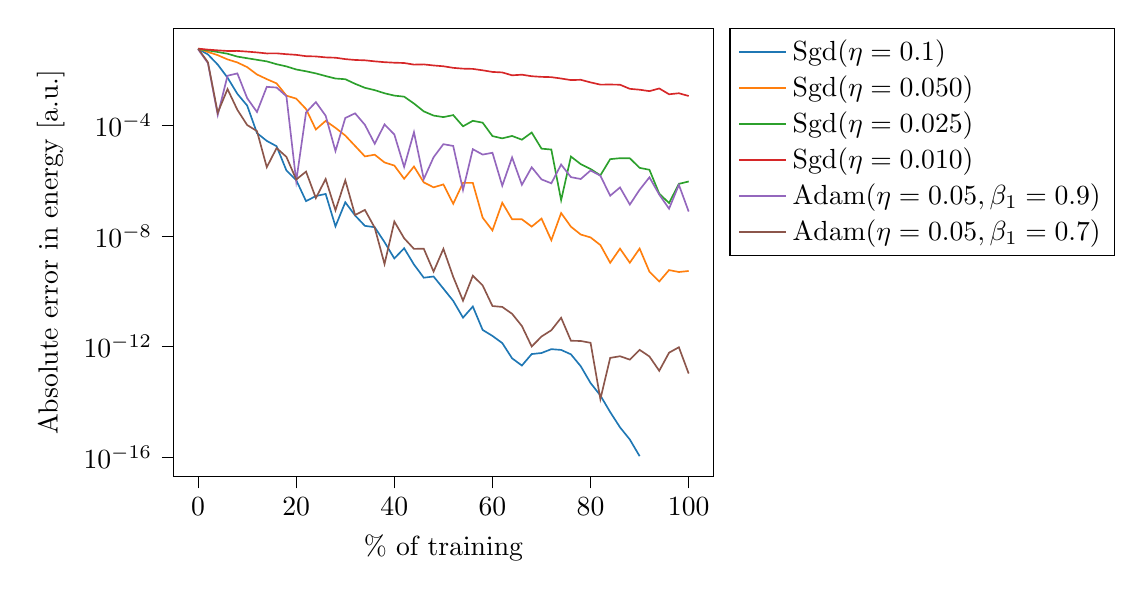
\begin{tikzpicture}

\definecolor{color0}{rgb}{0.12156862745098,0.466666666666667,0.705882352941177}
\definecolor{color1}{rgb}{1,0.498039215686275,0.0549019607843137}
\definecolor{color2}{rgb}{0.172549019607843,0.627450980392157,0.172549019607843}
\definecolor{color3}{rgb}{0.83921568627451,0.152941176470588,0.156862745098039}
\definecolor{color4}{rgb}{0.580392156862745,0.403921568627451,0.741176470588235}
\definecolor{color5}{rgb}{0.549019607843137,0.337254901960784,0.294117647058824}

\begin{axis}[
compat=newest,
legend cell align={left},
legend pos=outer north east,
log basis y={10},
tick align=outside,
tick pos=left,
x grid style={white!69.01960784313725!black},
xlabel={\% of training},
xmin=-2.5, xmax=52.5,
xtick style={color=black},
y grid style={white!69.01960784313725!black},
ylabel={Absolute error in energy [a.u.]},
ymin=2.04107850345761e-17, ymax=0.310435351581576,
ymode=log,
ytick style={color=black},
scaled x ticks={real:0.5},
xtick scale label code/.code={},
]
\addplot [semithick, color0]
table {%
0 0.055394637681096
1 0.0351704907386907
2 0.0150969846331099
3 0.00509220080030759
4 0.00133494835420322
5 0.000502231030251821
6 5.10133215083641e-05
7 2.66120006329196e-05
8 1.70668136009189e-05
9 2.27926573781456e-06
10 1.02116612221703e-06
11 1.78261272631985e-07
12 2.71528418804845e-07
13 3.23789623335458e-07
14 2.19051697891715e-08
15 1.62480448762103e-07
16 5.40524482950389e-08
17 2.28132451818297e-08
18 2.0413277734832e-08
19 5.88884296881531e-09
20 1.52055978919208e-09
21 3.54615325992569e-09
22 9.20566622930608e-10
23 3.06744407652104e-10
24 3.39281380767886e-10
25 1.23784205108279e-10
26 4.48276971098949e-11
27 1.10821352095059e-11
28 2.80035994393302e-11
29 4.00479649442786e-12
30 2.43155495738279e-12
31 1.34281474828413e-12
32 3.78364006792253e-13
33 2.07389660999979e-13
34 5.38458166943201e-13
35 5.87530024631633e-13
36 8.08797473439427e-13
37 7.59226015389913e-13
38 5.26023669067399e-13
39 1.95399252334028e-13
40 4.84612350248881e-14
41 1.72639680329212e-14
42 4.32986979603811e-15
43 1.22124532708767e-15
44 4.44089209850063e-16
45 1.11022302462516e-16
46 0
47 0
48 0
49 0
50 0
};
\addlegendentry{Sgd($\eta=0.1$)}
\addplot [semithick, color1]
table {%
0 0.0569362547036885
1 0.0432396488590304
2 0.0330463459171154
3 0.0232667815500573
4 0.0180607028034824
5 0.0122465985514122
6 0.00665045788563745
7 0.00451434225385761
8 0.00316624791476239
9 0.00114417979036119
10 0.000893183207241965
11 0.000376903798576245
12 6.86025596201567e-05
13 0.000140343631785278
14 7.89132510217172e-05
15 4.15745624122721e-05
16 1.75055080011699e-05
17 7.32614696508094e-06
18 8.45643669755702e-06
19 4.43285084655853e-06
20 3.43091891785718e-06
21 1.14237504644787e-06
22 3.16736307304222e-06
23 8.44236084818206e-07
24 5.60171690588973e-07
25 7.15364109615813e-07
26 1.43104883332246e-07
27 8.17226734950438e-07
28 8.10643462190175e-07
29 4.51685145397285e-08
30 1.56366360970495e-08
31 1.55801064827266e-07
32 3.95821858067968e-08
33 3.94758760124958e-08
34 2.14213821125853e-08
35 4.17884472025953e-08
36 6.91130469521184e-09
37 6.62794248373899e-08
38 2.12761959161867e-08
39 1.1105886321694e-08
40 8.72376748617398e-09
41 4.62737675954727e-09
42 1.05863218191615e-09
43 3.44135969720938e-09
44 1.06627157103745e-09
45 3.45928796718908e-09
46 5.06059694149741e-10
47 2.24251672786835e-10
48 5.7891913485264e-10
49 4.92443197330772e-10
50 5.36690913932603e-10
};
\addlegendentry{Sgd($\eta=0.050$)}
\addplot [semithick, color2]
table {%
0 0.0547455625405362
1 0.0491533822507542
2 0.0429889137691005
3 0.037280627197275
4 0.0293656333610928
5 0.0256417134312286
6 0.0224926209395288
7 0.0197289355419475
8 0.0156066369859533
9 0.0129890314612582
10 0.010076410599988
11 0.00866552932035602
12 0.00727475039578385
13 0.0058274087904211
14 0.00474640790013903
15 0.00448441120843224
16 0.00306308380954934
17 0.00219840578314923
18 0.00180795981297432
19 0.00139511421803651
20 0.00114810853498548
21 0.00105146335497286
22 0.000594045030576362
23 0.000309626328639068
24 0.000218461001944781
25 0.000192292335392641
26 0.000227070708281096
27 8.96098940986745e-05
28 0.000141304294990041
29 0.000121211029598944
30 3.9707419424051e-05
31 3.2820976388126e-05
32 4.01287951753426e-05
33 2.94069363704352e-05
34 5.33233073980455e-05
35 1.39630984149486e-05
36 1.29784259039756e-05
37 1.93103876333645e-07
38 7.24761540571439e-06
39 3.8541399401959e-06
40 2.57768717182305e-06
41 1.51772546652662e-06
42 5.8381873483393e-06
43 6.32328379779334e-06
44 6.28710736572113e-06
45 2.83606298934203e-06
46 2.41212200885466e-06
47 3.30873180853786e-07
48 1.52283458065838e-07
49 7.48224128876984e-07
50 9.12019611221115e-07
};
\addlegendentry{Sgd($\eta=0.025$)}
\addplot [semithick, color3]
table {%
0 0.0569021898367484
1 0.0524211232049313
2 0.0494035742277378
3 0.0468603945469587
4 0.0471072260701783
5 0.0444828571582362
6 0.0415456136773071
7 0.0382052245897901
8 0.0385269285628389
9 0.0358706949677516
10 0.0339674307781297
11 0.0303923626164787
12 0.0297605169401001
13 0.0274975901299466
14 0.0267665585146304
15 0.0238176191145419
16 0.0221988238805145
17 0.0215801617062573
18 0.0198185302462049
19 0.0184654747152159
20 0.0176828041037003
21 0.0172522325315738
22 0.0150872984394776
23 0.015352215821579
24 0.0140564006403868
25 0.013154874671103
26 0.011540612769255
27 0.0107866621601234
28 0.0105728439000026
29 0.00940407696767898
30 0.00821341094947381
31 0.00787682091465536
32 0.00620280826920716
33 0.00652578392915681
34 0.00574621099766903
35 0.00544671869047886
36 0.00532375137302044
37 0.00474527000724501
38 0.00417122296858363
39 0.00427424328214243
40 0.00344252162053615
41 0.00285848931104238
42 0.00288254515061315
43 0.00283673182931188
44 0.00201561735116462
45 0.00187543055338202
46 0.00166413474961291
47 0.00207974254233323
48 0.00128319300323232
49 0.00139673906994342
50 0.0011109425289193
};
\addlegendentry{Sgd($\eta=0.010$)}
\addplot [semithick, color4]
table {%
0 0.054060448912418
1 0.0171143276735576
2 0.000229283463824115
3 0.00598830356226754
4 0.00726830444938209
5 0.000929085035698551
6 0.000293933149466574
7 0.00237893445281734
8 0.00224313155783618
9 0.00109083910569285
10 9.29482563916117e-07
11 0.000283278257761199
12 0.000669134100598323
13 0.000215782855374713
14 1.14709657944578e-05
15 0.000178569751881907
16 0.000263464108337885
17 0.000101413325021116
18 2.10336165004099e-05
19 0.000104484336263755
20 4.52775760221291e-05
21 3.05896287977614e-06
22 5.49029916228072e-05
23 1.11507376598929e-06
24 6.85554842461134e-06
25 2.02741550152652e-05
26 1.75000688420468e-05
27 4.51828123582132e-07
28 1.33623192148935e-05
29 8.53124392252713e-06
30 9.91682775053349e-06
31 6.40266421769731e-07
32 6.73008228457839e-06
33 6.93101520843342e-07
34 2.96849921388453e-06
35 1.08708826995763e-06
36 7.84025391109555e-07
37 3.72679063209702e-06
38 1.30763228500808e-06
39 1.11987966483484e-06
40 2.28072352204123e-06
41 1.47374578540749e-06
42 2.79622188736894e-07
43 5.5594312226015e-07
44 1.34114747529779e-07
45 4.57867820158331e-07
46 1.29251660119234e-06
47 3.06874345212815e-07
48 9.51151273298478e-08
49 6.90530736646711e-07
50 7.48032291109091e-08
};
\addlegendentry{Adam($\eta=0.05,\beta_1=0.9$)}
\addplot [semithick, color5]
table {%
0 0.0570716791826928
1 0.0184088285463323
2 0.000275342452295102
3 0.00197419918807029
4 0.00035195477419292
5 9.95087981424669e-05
6 6.01126708595912e-05
7 2.99174000434332e-06
8 1.46416943125338e-05
9 7.06142390438647e-06
10 1.07239916780077e-06
11 2.07564791582238e-06
12 2.30205721374332e-07
13 1.12002768004604e-06
14 8.33629580920814e-08
15 1.00684648851601e-06
16 5.62263295367238e-08
17 8.58445727280888e-08
18 1.96012995834494e-08
19 9.54294421262603e-10
20 3.26812138462529e-08
21 8.1398958684531e-09
22 3.37213379442147e-09
23 3.40726835634797e-09
24 5.1158344227531e-10
25 3.37396072191964e-09
26 3.31022376176549e-10
27 4.54031257035581e-11
28 3.61375818158649e-10
29 1.62010294069148e-10
30 2.91066060142953e-11
31 2.70650168943121e-11
32 1.52768353522958e-11
33 5.54001289287953e-12
34 1.00897068477934e-12
35 2.31692443009024e-12
36 3.8924419243358e-12
37 1.09855458063635e-11
38 1.62614366416847e-12
39 1.59561253099127e-12
40 1.37134748001699e-12
41 1.27675647831893e-14
42 3.91575660785293e-13
43 4.49196235763338e-13
44 3.3939517862791e-13
45 7.62945262522408e-13
46 4.40536496171262e-13
47 1.34003919072256e-13
48 6.03683769639929e-13
49 9.47297795761415e-13
50 1.06248343456627e-13
};
\addlegendentry{Adam($\eta=0.05,\beta_1=0.7$)}
\end{axis}

\end{tikzpicture}
    }
  \caption{\label{fig:verify-lr-gaussian}Example training progression using
    $\psi_G$ as trial wave function with different optimization schemes. With
    sufficient time, all algorithms tend towards zero error.}
\end{figure}

\subsubsection{More Complex Problem - $\psi_{RBM}$}

We run the same test as above, now with $\psi_{RBM}$ as the trial wave function
instead. We do this to illustrate a common pitfall of gradient based
optimization - local minima. \cref{fig:verify-lr-rbm} shows three runs
plateauing around an error $\sim 10^{-6}\si{\au}$. Interestingly, the worst
result is obtained with the middle most value of $\eta$. This shows the random
nature of SGD, in that it is quite unpredictable when and where we might get
stuck due to a local minimum. Repeating the same experiment with different random
seeds does not consistently reproduce this particular result.

Similarly, we see that one of the ADAM runs did in fact stumble on to a
different, better local minimum. While this is also subject to randomness, we
find that ADAM tends to be at least as good as SGD whenever we have more than
one parameter to learn. This is to be expected, as ADAM can account for
different scales and variability in the components of the parameter gradient.

\begin{figure}[h]
  \centering
    \resizebox{\linewidth}{!}{%
      % This file was created by matplotlib2tikz v0.7.4.
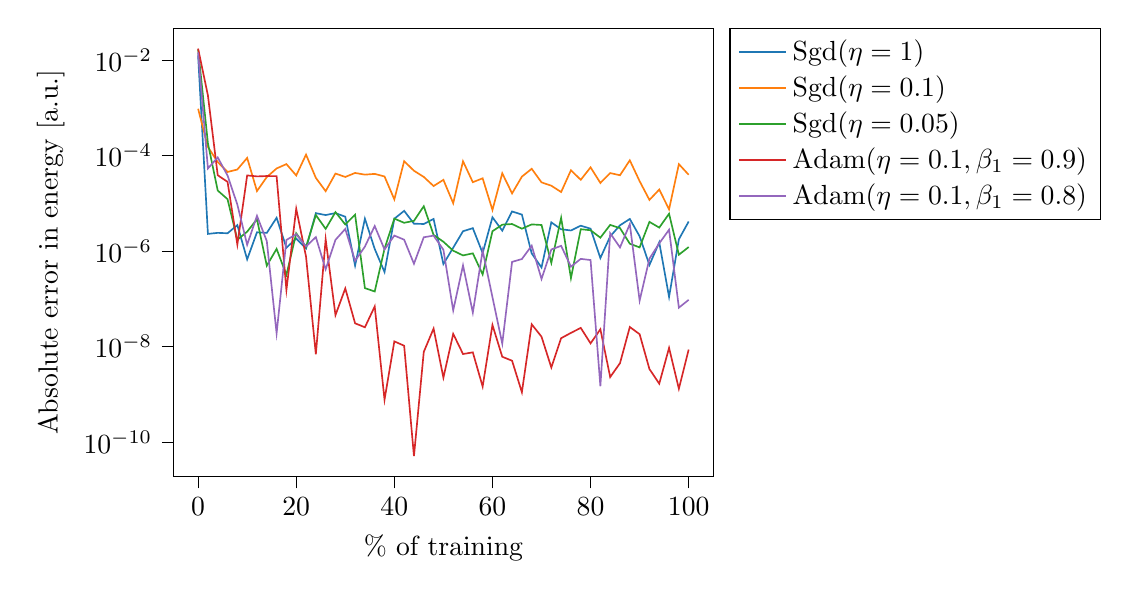
\begin{tikzpicture}

\definecolor{color0}{rgb}{0.12156862745098,0.466666666666667,0.705882352941177}
\definecolor{color1}{rgb}{1,0.498039215686275,0.0549019607843137}
\definecolor{color2}{rgb}{0.172549019607843,0.627450980392157,0.172549019607843}
\definecolor{color3}{rgb}{0.83921568627451,0.152941176470588,0.156862745098039}
\definecolor{color4}{rgb}{0.580392156862745,0.403921568627451,0.741176470588235}

\begin{axis}[
compat=newest,
legend cell align={left},
legend pos=outer north east,
log basis y={10},
tick align=outside,
tick pos=left,
x grid style={white!69.01960784313725!black},
xlabel={\% of training},
xmin=-2.5, xmax=52.5,
xtick style={color=black},
y grid style={white!69.01960784313725!black},
ylabel={Absolute error in energy [a.u.]},
ymin=1.88824350685265e-11, ymax=0.0459154775931012,
ymode=log,
ytick style={color=black},
scaled x ticks={real:0.5},
xtick scale label code/.code={},
]
\addplot [semithick, color0]
table {%
0 0.0124207570633597
1 2.26854526552689e-06
2 2.38681867392732e-06
3 2.34036513829805e-06
4 3.46659834249419e-06
5 6.65688472123449e-07
6 2.45183038150021e-06
7 2.37924669410639e-06
8 4.93323196087969e-06
9 1.16606802624819e-06
10 1.81452585457098e-06
11 1.11910005629046e-06
12 6.16845007084255e-06
13 5.62504728751634e-06
14 6.19087529762918e-06
15 5.19734613385614e-06
16 4.92239403460104e-07
17 4.72807347273729e-06
18 1.09942860260226e-06
19 3.61310680041527e-07
20 4.71271506496951e-06
21 6.89672227693894e-06
22 3.71240182150956e-06
23 3.65927889844908e-06
24 4.661996188704e-06
25 5.30933627396202e-07
26 1.16693677132407e-06
27 2.58022556065551e-06
28 2.99192052355401e-06
29 8.97729569016015e-07
30 5.05921433058276e-06
31 2.65325219800383e-06
32 6.69957468563132e-06
33 5.75843115291352e-06
34 8.85351812696111e-07
35 4.49372894950617e-07
36 3.95999965152605e-06
37 2.83616766405537e-06
38 2.67861462155405e-06
39 3.37156145974182e-06
40 2.9179329992246e-06
41 7.09094569950608e-07
42 2.01489764406482e-06
43 3.43788313100779e-06
44 4.66496526929649e-06
45 2.01911079478201e-06
46 5.06457129345605e-07
47 1.51084774835386e-06
48 1.08728200443053e-07
49 1.75004718916405e-06
50 4.12339146182994e-06
};
\addlegendentry{Sgd($\eta=1$)}
\addplot [semithick, color1]
table {%
0 0.000946764011007684
1 0.000149893587279903
2 7.25209884152589e-05
3 4.49589288755714e-05
4 5.06127766776165e-05
5 8.83735782755135e-05
6 1.7887840541686e-05
7 3.51331355303852e-05
8 5.32268838884242e-05
9 6.56656273740897e-05
10 3.79641174761414e-05
11 0.00010373003050701
12 3.37947102252434e-05
13 1.77824595075649e-05
14 4.16561995506548e-05
15 3.53237838244258e-05
16 4.28686565709935e-05
17 3.9496934066241e-05
18 4.09601322834963e-05
19 3.61866469791305e-05
20 1.19664381746931e-05
21 7.56282987967039e-05
22 4.76385067360585e-05
23 3.53823369725337e-05
24 2.28079706486861e-05
25 3.07140624435931e-05
26 9.9697780656105e-06
27 7.52885737179687e-05
28 2.74259545864908e-05
29 3.31136288921341e-05
30 7.19545992189374e-06
31 4.21025510261019e-05
32 1.59889967834559e-05
33 3.58598267145016e-05
34 5.24109413744256e-05
35 2.72187061834961e-05
36 2.31606226858139e-05
37 1.70835655144419e-05
38 4.87710266392494e-05
39 3.07893322754049e-05
40 5.61293133845009e-05
41 2.64682667254768e-05
42 4.26219964445584e-05
43 3.83737473698131e-05
44 7.87728906408436e-05
45 2.87985995551798e-05
46 1.1691915592138e-05
47 1.92440055311049e-05
48 7.42567528200233e-06
49 6.55030051638361e-05
50 3.92795360057985e-05
};
\addlegendentry{Sgd($\eta=0.1$)}
\addplot [semithick, color2]
table {%
0 0.0166644521412936
1 0.000179310394089138
2 1.83563633397998e-05
3 1.21008950048074e-05
4 1.71231418233386e-06
5 2.52634967257137e-06
6 4.60511930255869e-06
7 4.90692246113422e-07
8 1.10209128068028e-06
9 3.1458649574212e-07
10 2.33593877940752e-06
11 1.21441388795107e-06
12 5.63072029657885e-06
13 2.8935300286359e-06
14 6.48341261061391e-06
15 3.57210924040174e-06
16 5.71758548972845e-06
17 1.66433542614364e-07
18 1.4130442493876e-07
19 1.10972150069166e-06
20 4.74227001245886e-06
21 3.87464962159356e-06
22 4.25545038151842e-06
23 8.61836280907635e-06
24 2.16391680923911e-06
25 1.55424380388069e-06
26 1.01009437825095e-06
27 8.04049844538302e-07
28 8.88848610380855e-07
29 3.2209301015218e-07
30 2.57943256593007e-06
31 3.5430288728433e-06
32 3.655007074721e-06
33 2.91495795651242e-06
34 3.58616026946423e-06
35 3.4859093844819e-06
36 5.61612946925472e-07
37 4.92245395755653e-06
38 2.68988205598397e-07
39 2.84455200816325e-06
40 2.70801924773245e-06
41 1.89296412644868e-06
42 3.50476327287685e-06
43 2.99804393949499e-06
44 1.41438672762728e-06
45 1.1830302549809e-06
46 4.05199369235554e-06
47 3.07539620353348e-06
48 5.99579243165671e-06
49 8.31306203818993e-07
50 1.20401247377666e-06
};
\addlegendentry{Sgd($\eta=0.05$)}
\addplot [semithick, color3]
table {%
0 0.0171920330575592
1 0.00180000248024936
2 3.8397750563246e-05
3 2.79349201854906e-05
4 1.35389526501051e-06
5 3.80568843828533e-05
6 3.62791129472351e-05
7 3.69227051524312e-05
8 3.67072278122382e-05
9 1.52102793804509e-07
10 7.61985906871931e-06
11 7.59486060986081e-07
12 6.85757339802251e-09
13 1.75347602648923e-06
14 4.51800150624848e-08
15 1.6382421597072e-07
16 3.05018268975665e-08
17 2.51706008258523e-08
18 6.86196219845669e-08
19 7.66318841716185e-10
20 1.27624246171187e-08
21 1.0339799905168e-08
22 5.04301045367583e-11
23 7.69478292195203e-09
24 2.36251496144035e-08
25 2.21842144654261e-09
26 1.83245574270074e-08
27 6.93446244870444e-09
28 7.51389550579518e-09
29 1.44426703929668e-09
30 2.81390941658799e-08
31 6.07915212613719e-09
32 5.01788377516021e-09
33 1.09939335413145e-09
34 2.90264335345292e-08
35 1.60085535383381e-08
36 3.62025837086222e-09
37 1.48649075826235e-08
38 1.92233546858489e-08
39 2.44228502976895e-08
40 1.15894602803479e-08
41 2.28733257889857e-08
42 2.28381125122468e-09
43 4.46401537956831e-09
44 2.55023083761685e-08
45 1.80140987127153e-08
46 3.36027983216525e-09
47 1.66185348815517e-09
48 9.31843191498416e-09
49 1.29863808595587e-09
50 8.59386084517411e-09
};
\addlegendentry{Adam($\eta=0.1,\beta_1=0.9$)}
\addplot [semithick, color4]
table {%
0 0.0143350328962304
1 5.32499715006907e-05
2 9.05013938081733e-05
3 3.79302687117944e-05
4 9.31451076352507e-06
5 1.34435891196993e-06
6 5.43029427013675e-06
7 1.60861158626791e-06
8 1.88298219239158e-08
9 1.69261821858502e-06
10 2.23536690380222e-06
11 1.2384254835518e-06
12 1.94698265143511e-06
13 4.10142109052991e-07
14 1.70182267728025e-06
15 2.88102388723566e-06
16 6.20635117964952e-07
17 1.23034609805783e-06
18 3.32002507785756e-06
19 1.07119022019209e-06
20 2.09333788181443e-06
21 1.71771007628774e-06
22 5.38399077210094e-07
23 1.93036260831558e-06
24 2.08733074147371e-06
25 1.05755835549948e-06
26 5.68752549501284e-08
27 4.97479992089822e-07
28 5.10173275847237e-08
29 1.0134568338982e-06
30 1.07572733554218e-07
31 1.14403145845543e-08
32 5.88843373727777e-07
33 6.75575154818198e-07
34 1.28500117946295e-06
35 2.58369695305127e-07
36 1.07146356242982e-06
37 1.27713811459707e-06
38 4.67491970301825e-07
39 6.80996668500633e-07
40 6.43167457903271e-07
41 1.4704104045471e-09
42 2.33784446590501e-06
43 1.18207017762995e-06
44 3.63515377821422e-06
45 9.09971076823446e-08
46 6.88379101942971e-07
47 1.44008553570885e-06
48 2.77646201041204e-06
49 6.47876179371565e-08
50 9.44995167673213e-08
};
\addlegendentry{Adam($\eta=0.1,\beta_1=0.8$)}
\end{axis}

\end{tikzpicture}
    }
  \caption{\label{fig:verify-lr-rbm}Example training progression using
    $\psi_{RBM}$ as trial wave function with different optimization schemes. We
    see evidence of learning getting stuck in local minima due to the overly
    complex wave function anstaz.}
\end{figure}


\section{Sampling}

We will now investigate the behavior of the implemented sampling strategies.

\subsection{Step Dependency}

Similarly to the learning rate in optimization schemes, the Monte Carlo samplers
are highly dependent setting an appropriate step parameter. We want to use a 
step size that balances two opposing attributes:

\begin{itemize}
\item Particles should be sufficiently mobile.
  \begin{itemize}
  \item Unchanging configurations lead to biased energy estimates with high
    autocorrelation.
  \end{itemize}
\item New configurations should be accepted as much as possible.
  \begin{itemize}
  \item Rejections imply wasted computation time as well as increased autocorrelation.
  \end{itemize}
\end{itemize}


\cref{fig:verify-sampling-step} shows how the acceptance rate (AR) changes with
different step sizes. For both Metropolis and Importance sampling, the AR tends
to $\SI{100}{\percent}$ for low step sizes, and to $\SI{0}{\percent}$ for large
values. Both algorithms show a similar pattern in the middle region, with
a steeper decline for Importance sampling. A good trade-off between the above
considerations is achieved when the AR is somewhere in the range
\SIrange{50}{99}{\percent}, with the exact best value dependent on the
particular problem at hand.

\begin{figure}[h]
  \centering
    \resizebox{\linewidth}{!}{%
      % This file was created by matplotlib2tikz v0.7.4.
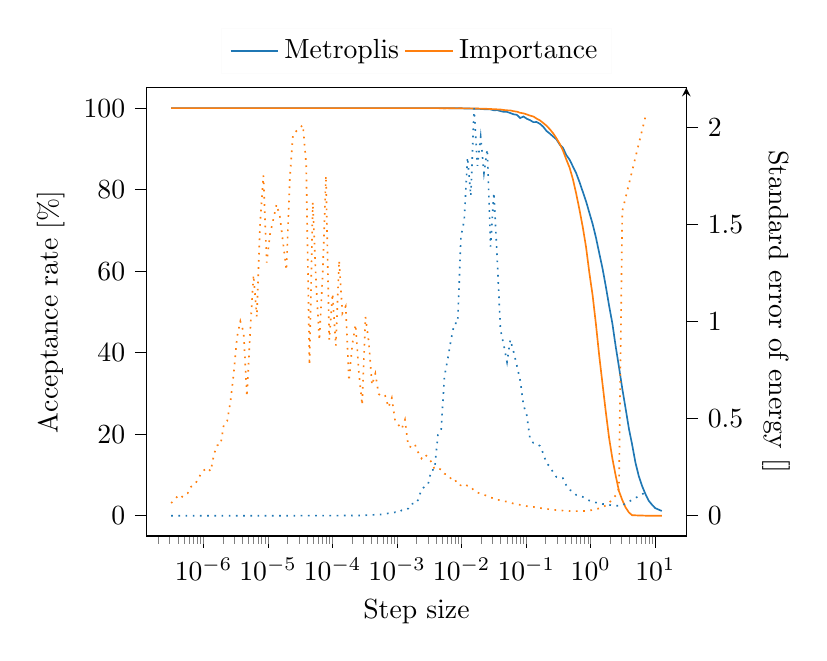
\begin{tikzpicture}

\definecolor{color0}{rgb}{0.12156862745098,0.466666666666667,0.705882352941177}
\definecolor{color1}{rgb}{1,0.498039215686275,0.0549019607843137}

\begin{axis}[
compat=newest,
legend cell align={left},
legend columns=2,
legend style={at={(0.5,1.03)}, anchor=south, draw=white!99.0!black},
log basis x={10},
tick align=outside,
tick pos=left,
x grid style={white!69.01960784313725!black},
xlabel={Step size},
xmin=1.31825673855641e-07, xmax=30.1995172040202,
xmode=log,
xtick style={color=black},
y grid style={white!69.01960784313725!black},
ylabel={Acceptance rate [\%]},
ymin=-5, ymax=105,
ytick style={color=black}
]
\addplot [semithick, color0]
table {%
3.16227766016838e-07 100
3.55636814392476e-07 100
3.99957111117477e-07 100
4.49800707518717e-07 100
5.05855930199755e-07 100
5.68896886645318e-07 100
6.39794155436576e-07 100
7.19526808706207e-07 100
8.09195932860095e-07 100
9.10039834283207e-07 100
1.02345114001628e-06 100
1.15099602955915e-06 100
1.29443586338654e-06 100
1.45575150686057e-06 100
1.6371706854463e-06 100
1.84119874899873e-06 100
2.07065326996762e-06 100
2.32870295331193e-06 100
2.61891139545953e-06 100
2.94528629661124e-06 100
3.31233480599822e-06 100
3.72512576439541e-06 100
4.18935970344355e-06 100
4.71144756845146e-06 100
5.29859925181914e-06 100
5.95892315970437e-06 100
6.70153818692179e-06 100
7.53669964641715e-06 100
8.47594089236926e-06 100
9.5322325926959e-06 100
1.07201618504746e-05 100
1.20561336478958e-05 100
1.35585973946364e-05 100
1.52483017092239e-05 100
1.71485809518541e-05 100
1.92856774656029e-05 100
2.1689103976096e-05 100
2.43920511542787e-05 100
2.74318459706162e-05 100
3.08504671704747e-05 100
3.46951249892556e-05 100
3.90189131129954e-05 100
4.3881541887829e-05 100
4.93501629037424e-05 100
5.55002963398924e-05 100
6.24168738778831e-05 100
7.01954115853485e-05 100
7.89433289670483e-05 100
8.87814323992139e-05 100
9.98455834329744e-05 100
0.000112288575005683 100
0.000126282241470109 100
0.000142019831580443 100
0.000159718677205389 100
0.000179623194622575 100
0.000202008259841328 100
0.00022718300456612 100
0.00025549508522191 100
0.000287335483995469 100
0.000323143908193779 100
0.000363414862483172 100
0.000408704477865214 100
0.000459638191695619 100
0.000516919384805205 100
0.00058133909499918 100
0.000653786941075581 99.998
0.000735263408220581 100
0.000826893664438683 100
0.000929943098818956 100
0.00104583479621657 100
0.00117616918967027 99.998
0.00132274616195038 99.996
0.00148758990145368 100
0.00167297685569848 99.998
0.00188146716844993 99.998
0.00211594003461396 99.996
0.00237963346114125 99.996
0.00267618898302862 100
0.00300970195193378 99.994
0.00338477809187557 99.99
0.00380659710303861 99.998
0.0042809841920339 99.99
0.00481449051642865 99.99
0.00541448365446283 99.982
0.00608924934931477 99.988
0.00684810593297632 99.972
0.00770153300990095 99.974
0.00866131617751056 99.948
0.00974070978211274 99.96
0.0109546199578431 99.918
0.0123198104763518 99.92
0.0138551342499618 99.874
0.0155817936852962 99.858
0.0175236334827868 99.836
0.0197074699255466 99.798
0.0221634612049965 99.736
0.0249255238973433 99.704
0.0280318013423359 99.678
0.0315251903924851 99.462
0.0354539338070102 99.51
0.0398722864713133 99.276
0.0448412646422928 99.086
0.0504294885663702 99.068
0.0567141301065598 98.786
0.0637819784650514 98.484
0.0717306387186525 98.346
0.0806698797185343 97.564
0.090723149968419 97.944
0.102029282415072 97.384
0.114744411693799 97.042
0.129044130305587 96.554
0.145125913502114 96.582
0.163211846365641 96.142
0.183551690744006 95.418
0.20642633439429 94.382
0.232151669966869 93.746
0.261082957397595 93.02
0.293619729951553 92.338
0.330211311669543 91.062
0.371363022411713 90.244
0.41764315618835 88.484
0.469690829146657 87.36
0.528224805592129 85.686
0.594053423929468 84.034
0.668085759597624 81.878
0.751344179156061 79.51
0.844978458890809 77.134
0.950281662914412 74.328
1.06870800003208 71.576
1.20189290597247 68.272
1.35167562831344 64.45
1.52012462599424 60.68
1.70956613417482 56.274
1.92261628891506 51.528
2.16221725530713 47.134
2.43167785798078 41.544
2.73471927507768 36.482
3.07552642671656 31.18
3.45880576760964 26.374
3.88985028193102 21.436
4.37461257799848 17.416
4.91978709218657 13.03
5.53290253728475 9.766
6.22242587198754 7.33
6.99787922730712 5.382
7.86997140463077 3.7
8.85074576137548 2.718
9.95374652650102 1.864
11.1942058426536 1.502
12.5892541179417 1.16
};
\addlegendentry{Metroplis}
\addplot [semithick, color1]
table {%
3.16227766016838e-07 100
3.55636814392476e-07 100
3.99957111117477e-07 100
4.49800707518717e-07 100
5.05855930199755e-07 100
5.68896886645318e-07 100
6.39794155436576e-07 100
7.19526808706207e-07 100
8.09195932860095e-07 100
9.10039834283207e-07 100
1.02345114001628e-06 100
1.15099602955915e-06 100
1.29443586338654e-06 100
1.45575150686057e-06 100
1.6371706854463e-06 100
1.84119874899873e-06 100
2.07065326996762e-06 100
2.32870295331193e-06 100
2.61891139545953e-06 100
2.94528629661124e-06 100
3.31233480599822e-06 100
3.72512576439541e-06 100
4.18935970344355e-06 100
4.71144756845146e-06 100
5.29859925181914e-06 100
5.95892315970437e-06 100
6.70153818692179e-06 100
7.53669964641715e-06 100
8.47594089236926e-06 100
9.5322325926959e-06 100
1.07201618504746e-05 100
1.20561336478958e-05 100
1.35585973946364e-05 100
1.52483017092239e-05 100
1.71485809518541e-05 100
1.92856774656029e-05 100
2.1689103976096e-05 100
2.43920511542787e-05 100
2.74318459706162e-05 100
3.08504671704747e-05 100
3.46951249892556e-05 100
3.90189131129954e-05 100
4.3881541887829e-05 100
4.93501629037424e-05 100
5.55002963398924e-05 100
6.24168738778831e-05 100
7.01954115853485e-05 100
7.89433289670483e-05 100
8.87814323992139e-05 100
9.98455834329744e-05 100
0.000112288575005683 100
0.000126282241470109 100
0.000142019831580443 100
0.000159718677205389 100
0.000179623194622575 100
0.000202008259841328 100
0.00022718300456612 100
0.00025549508522191 100
0.000287335483995469 100
0.000323143908193779 100
0.000363414862483172 100
0.000408704477865214 100
0.000459638191695619 100
0.000516919384805205 99.998
0.00058133909499918 99.998
0.000653786941075581 100
0.000735263408220581 100
0.000826893664438683 100
0.000929943098818956 99.996
0.00104583479621657 100
0.00117616918967027 99.996
0.00132274616195038 99.994
0.00148758990145368 99.996
0.00167297685569848 100
0.00188146716844993 99.996
0.00211594003461396 99.998
0.00237963346114125 99.992
0.00267618898302862 99.998
0.00300970195193378 99.992
0.00338477809187557 99.992
0.00380659710303861 99.996
0.0042809841920339 99.99
0.00481449051642865 99.972
0.00541448365446283 99.984
0.00608924934931477 99.974
0.00684810593297632 99.962
0.00770153300990095 99.948
0.00866131617751056 99.94
0.00974070978211274 99.966
0.0109546199578431 99.928
0.0123198104763518 99.932
0.0138551342499618 99.936
0.0155817936852962 99.906
0.0175236334827868 99.9
0.0197074699255466 99.864
0.0221634612049965 99.836
0.0249255238973433 99.822
0.0280318013423359 99.78
0.0315251903924851 99.732
0.0354539338070102 99.696
0.0398722864713133 99.658
0.0448412646422928 99.536
0.0504294885663702 99.46
0.0567141301065598 99.432
0.0637819784650514 99.24
0.0717306387186525 99.132
0.0806698797185343 98.848
0.090723149968419 98.714
0.102029282415072 98.452
0.114744411693799 98.148
0.129044130305587 97.942
0.145125913502114 97.418
0.163211846365641 96.986
0.183551690744006 96.346
0.20642633439429 95.686
0.232151669966869 94.812
0.261082957397595 93.824
0.293619729951553 92.604
0.330211311669543 91.252
0.371363022411713 89.552
0.41764315618835 87.408
0.469690829146657 85.4
0.528224805592129 82.57
0.594053423929468 79.042
0.668085759597624 75.088
0.751344179156061 70.828
0.844978458890809 65.904
0.950281662914412 59.616
1.06870800003208 54.024
1.20189290597247 47.006
1.35167562831344 39.254
1.52012462599424 32.34
1.70956613417482 25.466
1.92261628891506 19.076
2.16221725530713 14.006
2.43167785798078 9.84
2.73471927507768 6.022
3.07552642671656 3.84
3.45880576760964 2.034
3.88985028193102 0.8
4.37461257799848 0.112
4.91978709218657 0.088
5.53290253728475 0.04
6.22242587198754 0.038
6.99787922730712 0
7.86997140463077 0
8.85074576137548 0
9.95374652650102 0
11.1942058426536 0
12.5892541179417 0
};
\addlegendentry{Importance}
\end{axis}

\begin{axis}[
compat=newest,
axis y line=right,
log basis x={10},
tick align=outside,
x grid style={white!69.01960784313725!black},
xmin=1.31825673855641e-07, xmax=30.1995172040202,
xmode=log,
xtick pos=left,
xmajorticks=false,
y grid style={white!69.01960784313725!black},
ylabel={Standard error of energy [$\si{\centi\au}$]},
ylabel style={rotate=-180},
ymin=-0.00104904918108588, ymax=0.0220300332326274,
ytick pos=right,
yticklabel pos=left,
ytick style={color=black},
ytick scale label code/.code={},
]
\addplot [semithick, color0, dotted]
table {%
3.16227766016838e-07 1.95374490517342e-11
3.55636814392476e-07 3.43002756216893e-11
3.99957111117477e-07 3.27982537353495e-11
4.49800707518717e-07 5.54537809915603e-11
5.05855930199755e-07 5.70907159718558e-11
5.68896886645318e-07 8.18132745879044e-11
6.39794155436576e-07 7.47704759773976e-11
7.19526808706207e-07 1.11416431064185e-10
8.09195932860095e-07 1.63923115541449e-10
9.10039834283207e-07 1.80521324187058e-10
1.02345114001628e-06 2.05824065227296e-10
1.15099602955915e-06 2.20895889699791e-10
1.29443586338654e-06 3.23261500343751e-10
1.45575150686057e-06 4.55027066928157e-10
1.6371706854463e-06 4.45357620765015e-10
1.84119874899873e-06 8.0442050891913e-10
2.07065326996762e-06 9.46849972989172e-10
2.32870295331193e-06 7.99268579308075e-10
2.61891139545953e-06 1.70884742279042e-09
2.94528629661124e-06 1.85857921442276e-09
3.31233480599822e-06 1.65309427299966e-09
3.72512576439541e-06 3.21651067019241e-09
4.18935970344355e-06 4.23858173300924e-09
4.71144756845146e-06 4.41473389277437e-09
5.29859925181914e-06 6.44482306392391e-09
5.95892315970437e-06 8.50702456949258e-09
6.70153818692179e-06 1.05960116900145e-08
7.53669964641715e-06 9.08793867785842e-09
8.47594089236926e-06 1.67541175967783e-08
9.5322325926959e-06 2.00955794982513e-08
1.07201618504746e-05 2.06973317579806e-08
1.20561336478958e-05 2.93940303111606e-08
1.35585973946364e-05 3.69073563887816e-08
1.52483017092239e-05 5.21846319451639e-08
1.92856774656029e-05 6.80897229323639e-08
2.1689103976096e-05 9.8321762113325e-08
2.43920511542787e-05 1.40117210303356e-07
3.46951249892556e-05 2.98603416920718e-07
3.90189131129954e-05 2.95615092578032e-07
4.3881541887829e-05 4.46827851284306e-07
4.93501629037424e-05 4.46985551197982e-07
5.55002963398924e-05 9.06971563165282e-07
6.24168738778831e-05 1.11198399691471e-06
7.01954115853485e-05 1.20761092632597e-06
7.89433289670483e-05 1.37106095989651e-06
8.87814323992139e-05 1.78815870297178e-06
9.98455834329744e-05 2.61295158477227e-06
0.000112288575005683 2.17109857266777e-06
0.000126282241470109 3.09545005345716e-06
0.000142019831580443 5.43176658119195e-06
0.000159718677205389 5.94702211031182e-06
0.000179623194622575 8.14755186663983e-06
0.000202008259841328 9.52438196082651e-06
0.00022718300456612 1.26084075997003e-05
0.00025549508522191 1.24096203506904e-05
0.000287335483995469 1.32636151912346e-05
0.000323143908193779 2.20856892402258e-05
0.000363414862483172 3.66069509421475e-05
0.000408704477865214 4.12032871723326e-05
0.000459638191695619 4.54875636357516e-05
0.000516919384805205 6.40179721048777e-05
0.00058133909499918 6.427284446675e-05
0.000653786941075581 9.83837243555054e-05
0.000735263408220581 0.000121868905748326
0.000826893664438683 0.000145161436659679
0.000929943098818956 0.000173572018933999
0.00104583479621657 0.000153113280298409
0.00117616918967027 0.000275007835392218
0.00132274616195038 0.000272926480941083
0.00148758990145368 0.000369180688334433
0.00167297685569848 0.000623609504808272
0.00188146716844993 0.000595912784066208
0.00211594003461396 0.000810483205053105
0.00237963346114125 0.00135350927777971
0.00267618898302862 0.0014908902072418
0.00300970195193378 0.00160030514997907
0.00338477809187557 0.0023323985168677
0.00380659710303861 0.00238708819554381
0.0042809841920339 0.00414868754358507
0.00481449051642865 0.00445531025303613
0.00541448365446283 0.00718160075271778
0.00608924934931477 0.00807307985417246
0.00684810593297632 0.00906391786283732
0.00770153300990095 0.00989872343098109
0.00866131617751056 0.00990949267084789
0.00974070978211274 0.0143540464911211
0.0109546199578431 0.0152141744260996
0.0123198104763518 0.0184483921544579
0.0138551342499618 0.0164676442929241
0.0155817936852962 0.020980984032004
0.0175236334827868 0.01800631070245
0.0197074699255466 0.0195011258237126
0.0221634612049965 0.0176431603887294
0.0249255238973433 0.0188645632268927
0.0280318013423359 0.0138567619001524
0.0315251903924851 0.0166277851626212
0.0354539338070102 0.0132959447067316
0.0398722864713133 0.00958903309330776
0.0448412646422928 0.00878106456816651
0.0504294885663702 0.00790717073950574
0.0567141301065598 0.00906047936587658
0.0637819784650514 0.00843317720535894
0.0717306387186525 0.00772241346026853
0.0806698797185343 0.00695667971516343
0.090723149968419 0.00568392306351504
0.102029282415072 0.00516400149620841
0.114744411693799 0.00392491609469204
0.129044130305587 0.00374449406607848
0.145125913502114 0.00370019016480751
0.163211846365641 0.00358822828711983
0.183551690744006 0.003201353940096
0.20642633439429 0.0026926158476611
0.232151669966869 0.002538961099897
0.261082957397595 0.00223045626308777
0.293619729951553 0.00199082815566909
0.330211311669543 0.00192649743518655
0.371363022411713 0.00192812191431867
0.41764315618835 0.00156416788814937
0.469690829146657 0.00132902630654337
0.528224805592129 0.00124559937378021
0.594053423929468 0.00106658331072967
0.668085759597624 0.0010121616085692
0.751344179156061 0.000967619853327907
0.844978458890809 0.000866669573338799
0.950281662914412 0.000778970333669307
1.06870800003208 0.000733679122523221
1.20189290597247 0.000675662403833159
1.35167562831344 0.000656133643615646
1.52012462599424 0.000602802673462973
1.70956613417482 0.000589639503336485
1.92261628891506 0.000562675778937507
2.16221725530713 0.000516845563793576
2.43167785798078 0.000512831112668849
2.73471927507768 0.000509695118875764
3.07552642671656 0.000531821552904698
6.99787922730712 0.00119377955092338
};
\addplot [semithick, color1, dotted]
table {%
3.16227766016838e-07 0.000648215920851033
3.55636814392476e-07 0.000821145604626832
3.99957111117477e-07 0.0010145372894497
4.49800707518717e-07 0.000912047394540926
5.05855930199755e-07 0.00111336855189366
5.68896886645318e-07 0.00115283007989224
6.39794155436576e-07 0.00148621940582313
7.19526808706207e-07 0.00158162772180051
8.09195932860095e-07 0.00182227887699088
9.10039834283207e-07 0.00214858914189422
1.02345114001628e-06 0.00234383040281676
1.15099602955915e-06 0.00246738987102627
1.29443586338654e-06 0.00228599319991456
1.45575150686057e-06 0.00316803763264181
1.6371706854463e-06 0.00362358381775556
1.84119874899873e-06 0.00365599707611082
2.07065326996762e-06 0.00470389771563708
2.32870295331193e-06 0.00487234542823428
2.61891139545953e-06 0.00586830161125088
2.94528629661124e-06 0.00734651715673676
3.31233480599822e-06 0.00919606574252815
3.72512576439541e-06 0.0100077937174853
4.18935970344355e-06 0.00943673915572927
4.71144756845146e-06 0.00613872094308711
5.29859925181914e-06 0.00950721024005696
5.95892315970437e-06 0.0123890803456419
6.70153818692179e-06 0.0102277521099682
7.53669964641715e-06 0.0149929339328937
8.47594089236926e-06 0.0175164935353034
9.5322325926959e-06 0.0130307676630192
1.07201618504746e-05 0.014474694694274
1.20561336478958e-05 0.0152368662449186
1.35585973946364e-05 0.0160214179290114
1.52483017092239e-05 0.0154065319077215
1.92856774656029e-05 0.0126392035409565
2.1689103976096e-05 0.0172953415803129
2.43920511542787e-05 0.0196383104627947
3.46951249892556e-05 0.0201118981224812
3.90189131129954e-05 0.0180905472064343
4.3881541887829e-05 0.00776558264305161
4.93501629037424e-05 0.0161407012356812
5.55002963398924e-05 0.0120073334790605
6.24168738778831e-05 0.00903445553306863
7.01954115853485e-05 0.0124191992439468
7.89433289670483e-05 0.0175015854924134
8.87814323992139e-05 0.00904637227241532
9.98455834329744e-05 0.0114298101327493
0.000112288575005683 0.00874225732255313
0.000126282241470109 0.0131259649521003
0.000142019831580443 0.0104213887468283
0.000159718677205389 0.0107769177307078
0.000179623194622575 0.0069295105613254
0.000202008259841328 0.00881033589510424
0.00022718300456612 0.00984096875521725
0.00025549508522191 0.00738640274386428
0.000287335483995469 0.0057004764777771
0.000323143908193779 0.0102335268432184
0.000363414862483172 0.00895522432204377
0.000408704477865214 0.00672784805041727
0.000459638191695619 0.00731363326420882
0.000516919384805205 0.00626844149651238
0.00058133909499918 0.00611840792133654
0.000653786941075581 0.00616607375147765
0.000735263408220581 0.00557656990536883
0.000826893664438683 0.00605319355929047
0.000929943098818956 0.00489346293319505
0.00104583479621657 0.00468033083418302
0.00117616918967027 0.00445989261080221
0.00132274616195038 0.00493699752327475
0.00148758990145368 0.00358334960676307
0.00167297685569848 0.00352496772055518
0.00188146716844993 0.00367564708163528
0.00211594003461396 0.00326630906408939
0.00237963346114125 0.00294630324198073
0.00267618898302862 0.00316054520048279
0.00300970195193378 0.00300768419941736
0.00338477809187557 0.00276366176822644
0.00380659710303861 0.00239429123841658
0.0042809841920339 0.00241844857330509
0.00481449051642865 0.00238519508380258
0.00541448365446283 0.00215641287486348
0.00608924934931477 0.00211017175812581
0.00684810593297632 0.00189926640732546
0.00770153300990095 0.00192249392260237
0.00866131617751056 0.00158709210253168
0.00974070978211274 0.00156459624054993
0.0109546199578431 0.00163895918029887
0.0123198104763518 0.00153826363113747
0.0138551342499618 0.00150384287464528
0.0155817936852962 0.0012756936581657
0.0175236334827868 0.00118842785179379
0.0197074699255466 0.00114085989302186
0.0221634612049965 0.00107150044524851
0.0249255238973433 0.00101462265798245
0.0280318013423359 0.000925607761643237
0.0315251903924851 0.000899450022101569
0.0354539338070102 0.000820342171250158
0.0398722864713133 0.000796341296801802
0.0448412646422928 0.000746853552064538
0.0504294885663702 0.000721460647152803
0.0567141301065598 0.00067100036541782
0.0637819784650514 0.000620386239534011
0.0717306387186525 0.000584332778240377
0.0806698797185343 0.000555372702136437
0.090723149968419 0.000527303518564487
0.102029282415072 0.000487849320664211
0.114744411693799 0.000454675575961289
0.129044130305587 0.000453027677109408
0.145125913502114 0.000409324615208452
0.163211846365641 0.000396578735809672
0.183551690744006 0.000367531472577131
0.20642633439429 0.000343158484622763
0.232151669966869 0.000331519222734867
0.261082957397595 0.000306288748617428
0.293619729951553 0.000288306307130755
0.330211311669543 0.000278058579355705
0.371363022411713 0.000258286983320561
0.41764315618835 0.000250372505043874
0.469690829146657 0.000241192695341119
0.528224805592129 0.000237688831438363
0.594053423929468 0.000234813683303625
0.668085759597624 0.000233326530478174
0.751344179156061 0.000240026074258359
0.844978458890809 0.000247853279378266
0.950281662914412 0.000271220629180144
1.06870800003208 0.000292023864124384
1.20189290597247 0.000339343068488174
1.35167562831344 0.000373625465953462
1.52012462599424 0.000445179872707595
1.70956613417482 0.000520780984795073
1.92261628891506 0.00065263938106288
2.16221725530713 0.000860514610138779
2.43167785798078 0.0010410529832615
2.73471927507768 0.00141478756557224
3.07552642671656 0.0156736012685009
6.99787922730712 0.0205134470666518
};
\end{axis}

\end{tikzpicture}
    }
    \caption{\label{fig:verify-sampling-step}\emph{Solid lines:} Acceptance rate of
    Metropolis and Importance sampling as a function of step size. Note that the
  interpretation of the step size is different for the two algorithms. \emph{Dashed
  lines:} Standard error of energy estimates obtained using the corresponding
  sampling algorithm and step size, using $\psi_G$ with $\alpha=0.51$.}
\end{figure}


The dotted lines show the standard error obtained using the
corresponding sampler and step size, when calculating the local energy with
$\psi_G$ and $\alpha=0.51$.\footnote{The value $\alpha=0.51$ was used to avoid
  the zero variance of the ideal value $\alpha=0.5$, but still behaving
  similarly to the real system.} The errors were calculated using $2^{21}$ MC
samples and corrected for autocorrelation using Blocking~\cite{Jonsson-2018}.

We see Metropolis tending to very small errors in the range shown, with a large
spike around $\delta \approx 0.01$. We believe step sizes around this critical
point allows enough movement for the system to randomly get into unlikely
states, but still so small that getting out of these states takes a long time,
leading to a significant portion of samples from unimportant states. The low
error for both high and low step sizes can be explained by both extremes
resulting in similar behavior; no effective change. When the system remains
unchanged, either from rejected samples or effectively equivalent ones (for high
and low step sizes, respectively), the resulting local energies must necessarily
be very similar as well. Neither case is desirable considering accurate
integration results. Recall that the standard error is a statistical measure of
the \emph{precision} of the local energy estimate, and not a measure of its
\emph{accuracy}.\footnote{The number $3.14159$ is more precise than the number
$6$, but if the true value is $6.28$, then the latter is more accurate.}\\

Importance sampling shows different behavior with respect to the standard error.
For the entire range of good step size choices, Importance sampling results in
smaller statistical errors. This is to be expected, and Importance sampling will
therefore be preferred whenever it is available to us.

Still, we would like to explain the behavior for non-optimal step sizes. The
error shows a spike as the step size decreases, in a similar way as seen for
Metropolis. Although not shown fully, the error also explodes once the
acceptance rate goes below a few percent. We believe this behavior is a result
of how the update rule for Importance sampling is dependent on both the step
size and its square root.

For small step sizes, the square root term will dominate, and the algorithm
effectively decays into standard Metropolis. The location of the spike is
shifted towards smaller step sizes (approximately the square of the Metropolis spike location),
and the spike is wider because the square root function grows slower than
linearly.

Finally, the unstable behavior for large step sizes can be explained the other
way. The little remaining movement is dominated by the drift force, and the
system will quickly get stuck in a local maximum of the wave function, and then be
unable to get out again. These are maxima with large probability amplitudes,
resulting in large values for the local energy and correspondingly large errors.

\end{document}
